\documentclass{beamer}

\usepackage[utf8x]{inputenc}
\usepackage{default}


\usepackage[utf8x]{inputenc}
\usepackage{listings}
\usepackage{graphicx}
\usepackage{caption}

\newcommand\Fontvi{\fontsize{6}{7.2}\selectfont}


\title{DISK SELF-GRAVITY CALCULATIONS ON A LEVEL 1 GRID WITH LEVEL 0 REFINEMENT}
\subtitle{Computational Science II - University of Zurich}
\author{Mihai Tomozeiu}
\date{4th June 2015}

\pdfinfo{%
  /Title    ()
  /Author   ()
  /Creator  ()
  /Producer ()
  /Subject  ()
  /Keywords ()
}

\begin{document}

\maketitle

\begin{frame}
 \frametitle{Contents}
\begin{itemize}
\item March starting point;
\item New approach;
\item Code schema; 
\item Results; 
\item Time measurements;
\item Towards a faster code;
\end{itemize}



%\begin{figure}
%\left
%\includegraphics[width = .4\textwidth]{}
%\includegraphics[width = .4\textwidth]{}    

%\caption{\label{fig:collage} The first/second column corresponds to the radial/tangetial component of the 
%acceleration due to relative self-gravity. First row displayes the values on a polar map, while the second displayes them on a rectangular grid for easier visualization. }
%\end{figure}


\end{frame}

\begin{frame}
\frametitle{March starting point}
\Fontvi

\begin{figure}
%\left
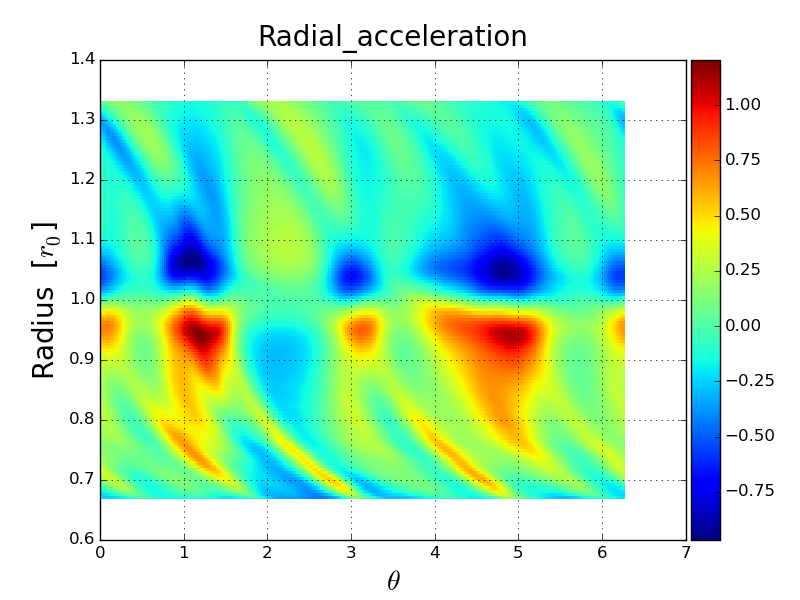
\includegraphics[width = .5\textwidth]{./Radial_acceleration_linear.png}
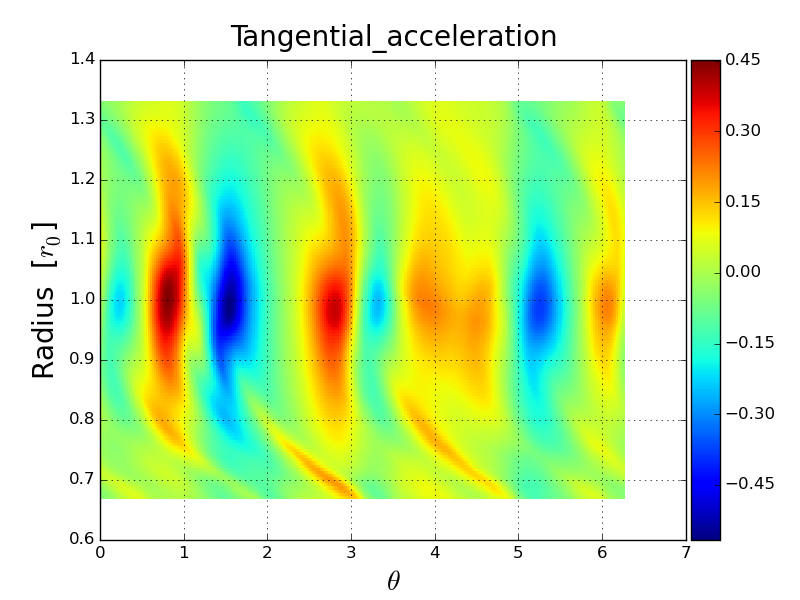
\includegraphics[width = .5\textwidth]{./Tangential_acceleration_linear.png} 
\newline   
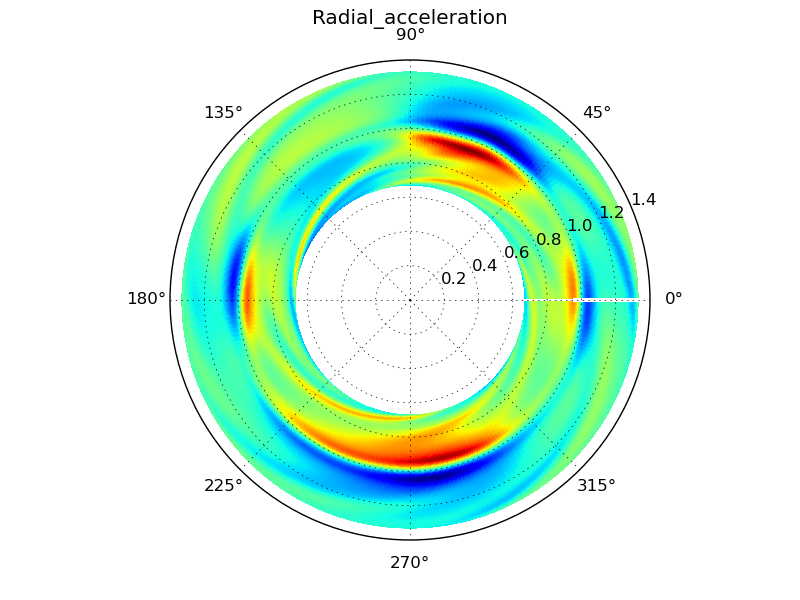
\includegraphics[width = .5\textwidth]{./Radial_acceleration_polar.png}
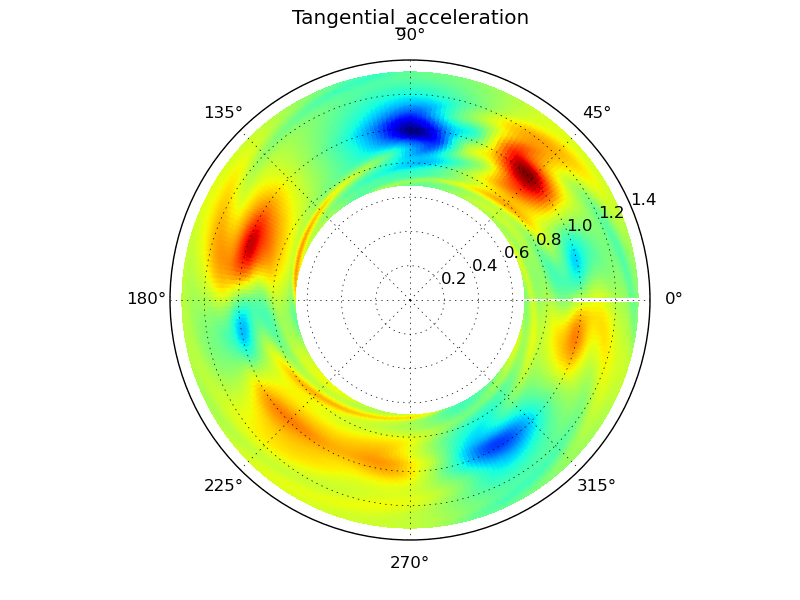
\includegraphics[width = .5\textwidth]{./Tangential_acceleration_polar.png}
%\caption{\label{fig:collage} The first/second column corresponds to the radial/tangetial component of the 
%acceleration due to relative self-gravity. First row displayes the values on a polar map, while the second displayes them on a rectangular grid for easier visualization. }
\end{figure}

\end{frame}

\begin{frame}
\frametitle{March starting point}
\Fontvi
\begin{figure}
 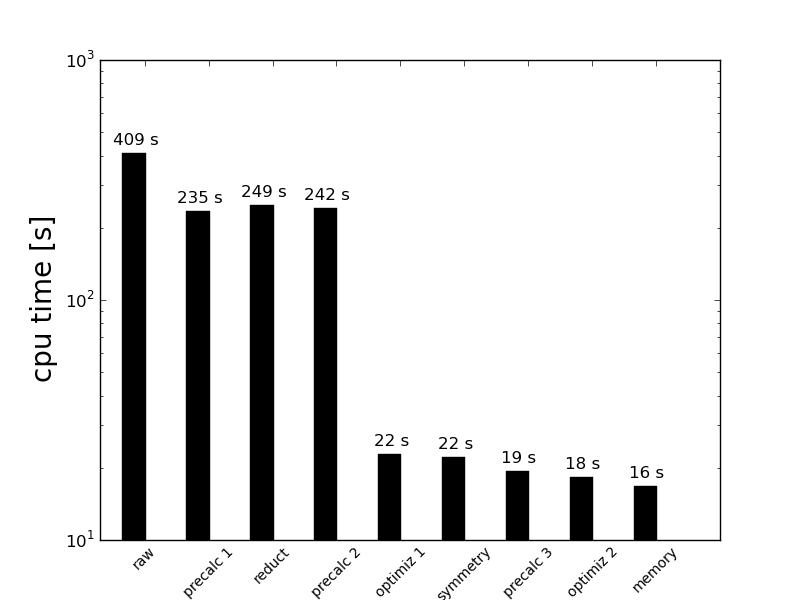
\includegraphics[width = .5\textwidth]{./time_plot.png}
\end{figure}

\begin{itemize}
\item reduction of the number of calculations;
\item a priori calculation of 1D and 2D arrays;
\item use of trigonometric relations;
\end{itemize}

\end{frame}

\begin{frame}
\frametitle{New approach}

\begin{figure}

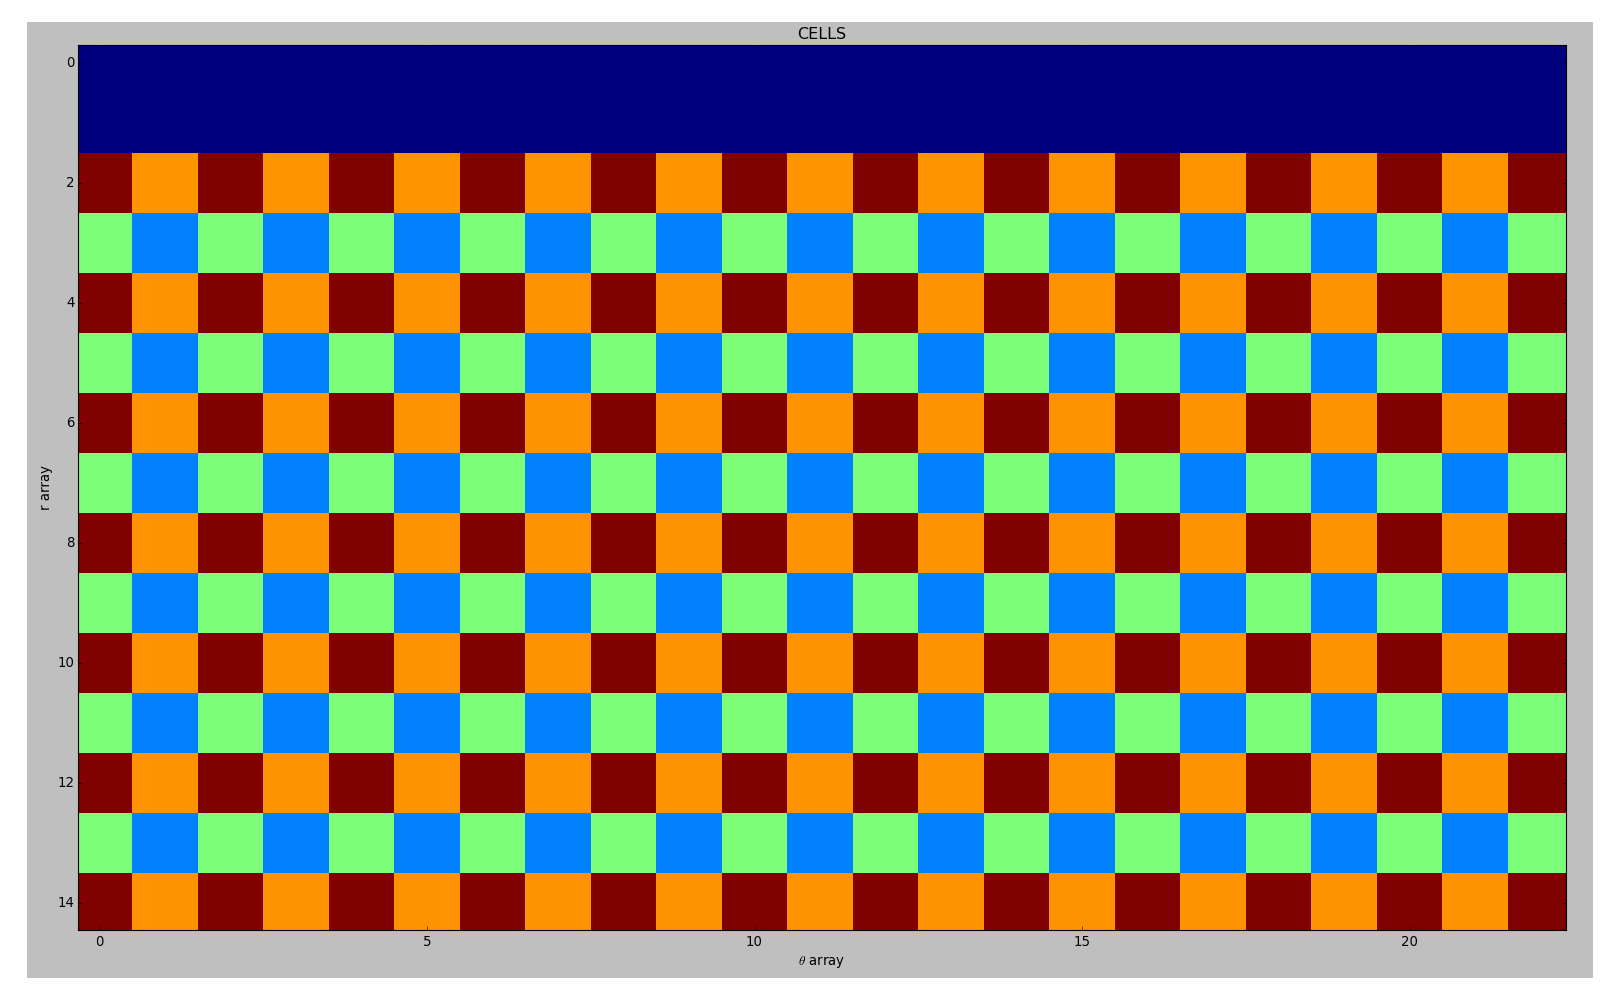
\includegraphics[width = \textwidth]{./cells.png}
%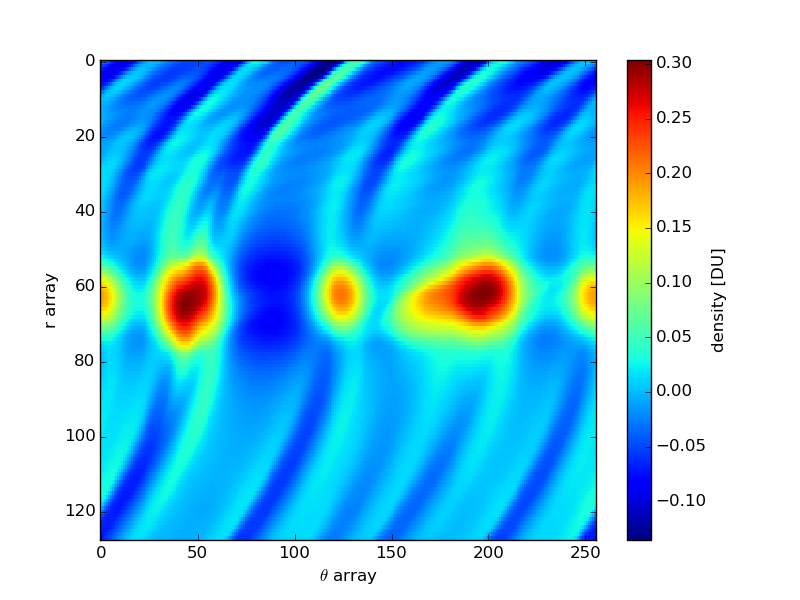
\includegraphics[width = .5\textwidth]{./density.png}

\caption{Cells coloured according to the parity of their indices.}
\end{figure}

\end{frame}


\begin{frame}
\frametitle{New approach}

\begin{figure}

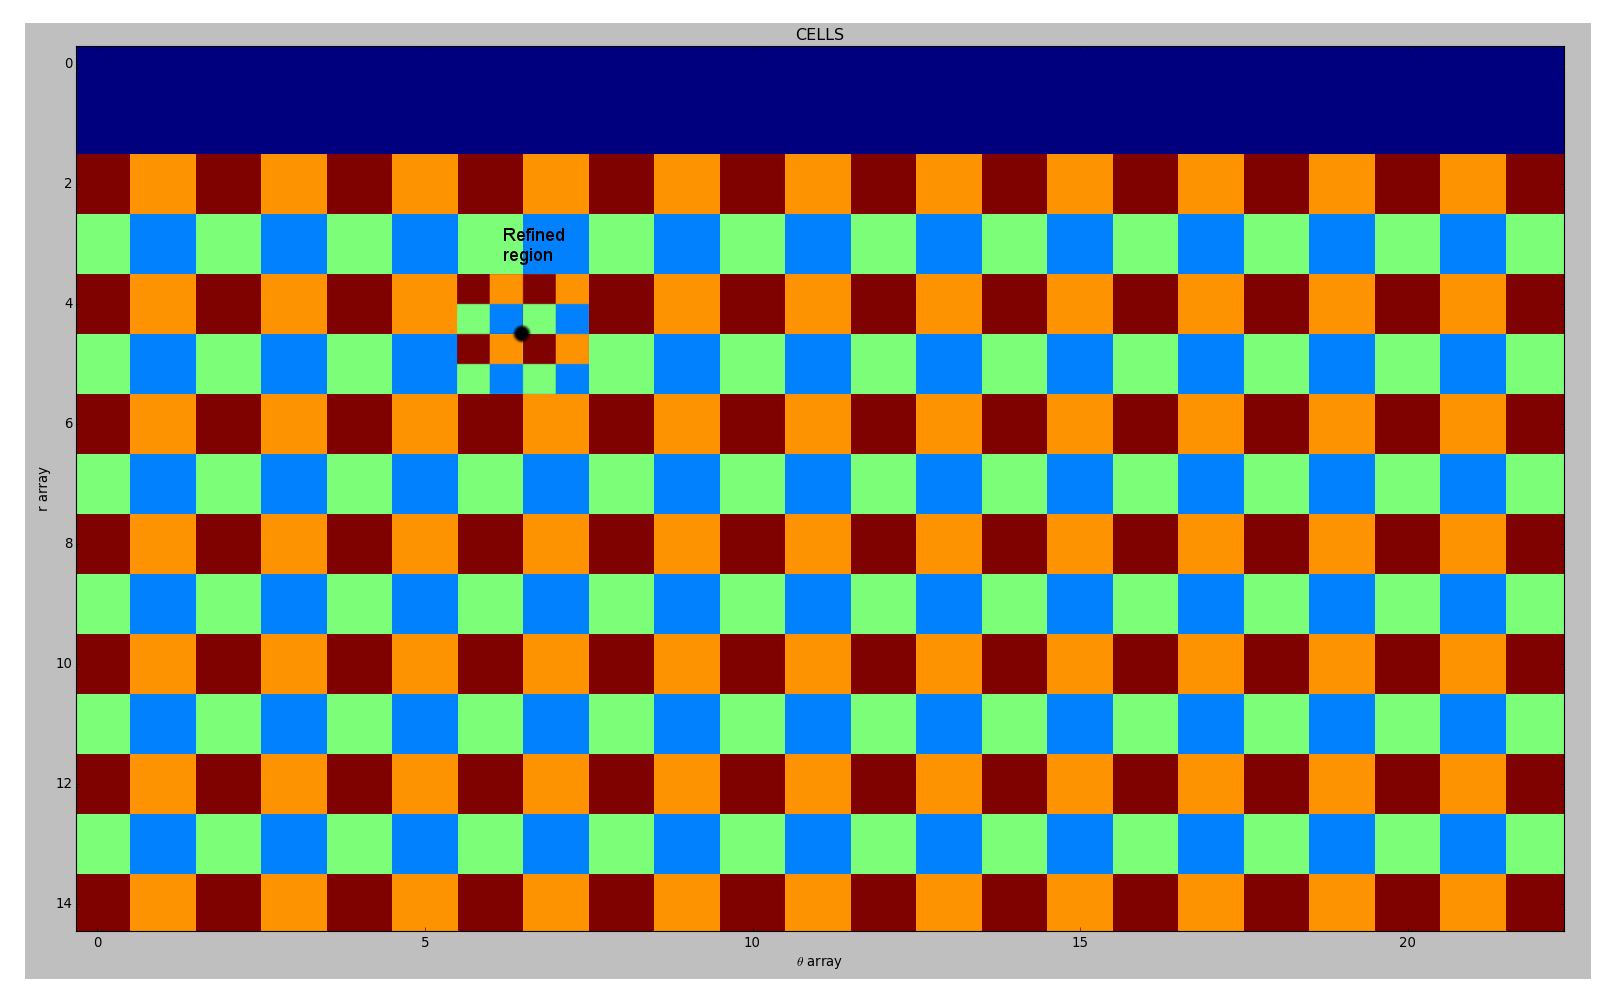
\includegraphics[width = \textwidth]{./cells_ref.png}
%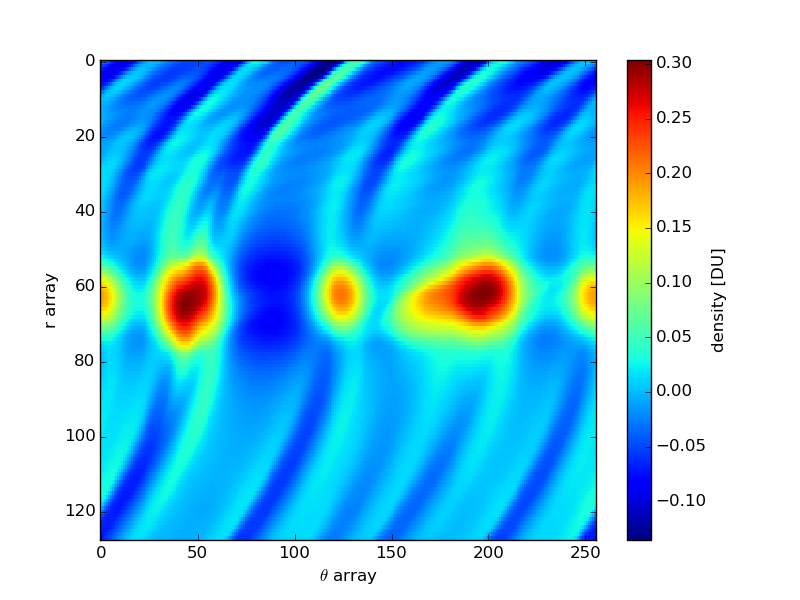
\includegraphics[width = .5\textwidth]{./density.png}

\caption{Refinement to the next lower level}
\end{figure}

\end{frame}



\begin{frame}
\frametitle{Code schema}

\begin{figure}

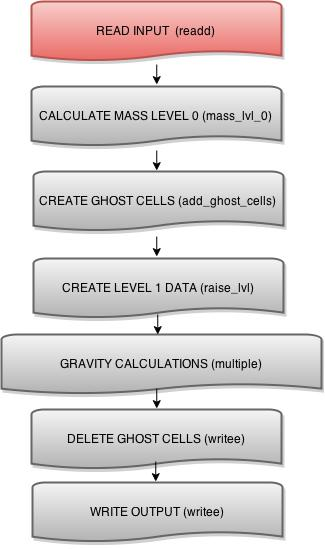
\includegraphics[width = .25\textwidth]{./Diagram1.jpg}
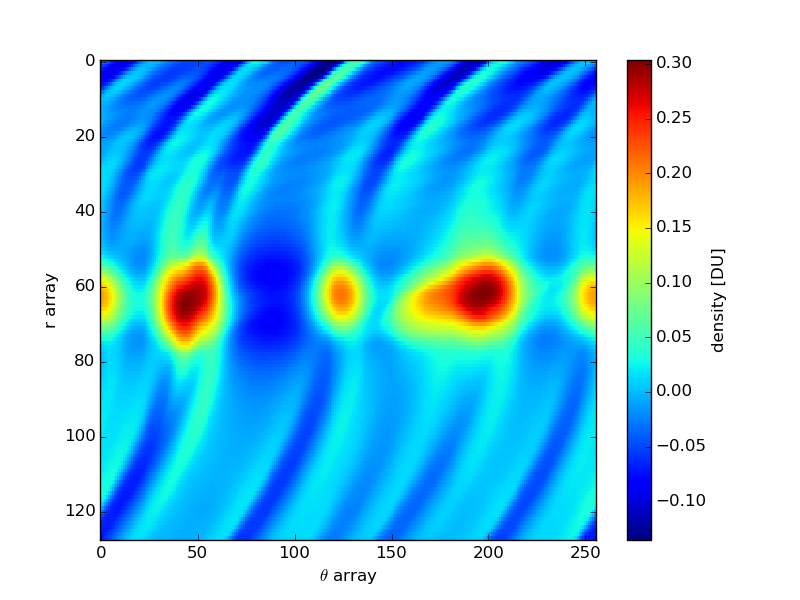
\includegraphics[width = .5\textwidth]{./density.png}
\end{figure}

\end{frame}


\begin{frame}
\frametitle{Code schema}

\begin{figure}

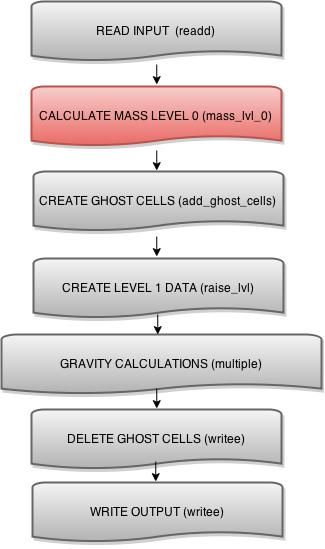
\includegraphics[width = .25\textwidth]{./Diagram2.jpg}
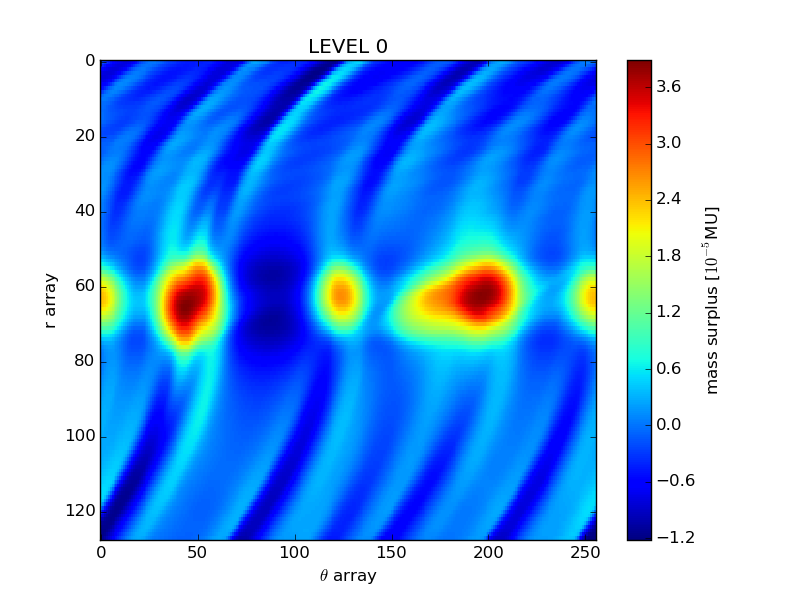
\includegraphics[width = .5\textwidth]{./mass.png}
\end{figure}

\end{frame}


\begin{frame}
\frametitle{Code schema}

\begin{figure}

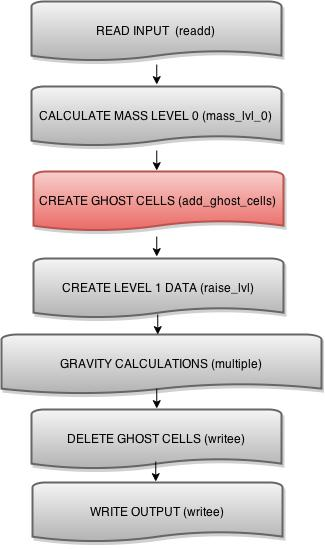
\includegraphics[width = .25\textwidth]{./Diagram3.jpg}
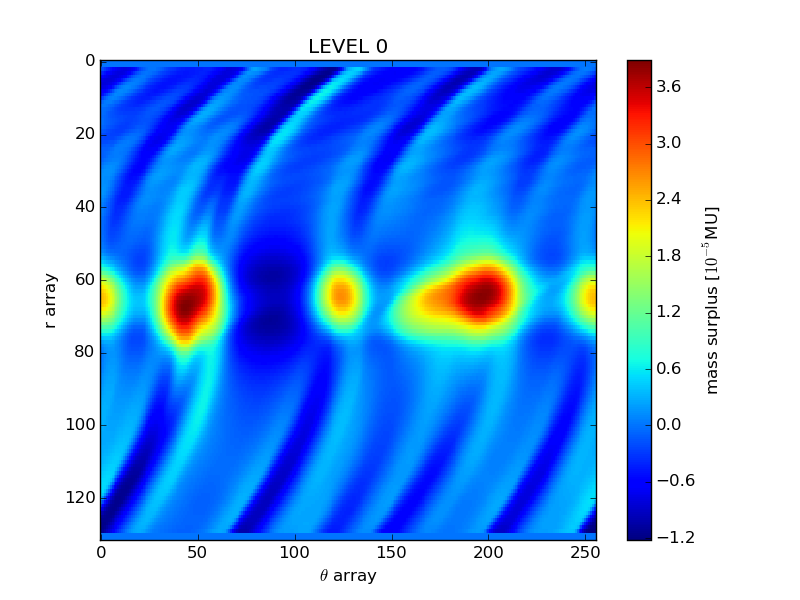
\includegraphics[width = .5\textwidth]{./mass_g.png}
\end{figure}

\end{frame}


\begin{frame}
\frametitle{Code schema}

\begin{figure}

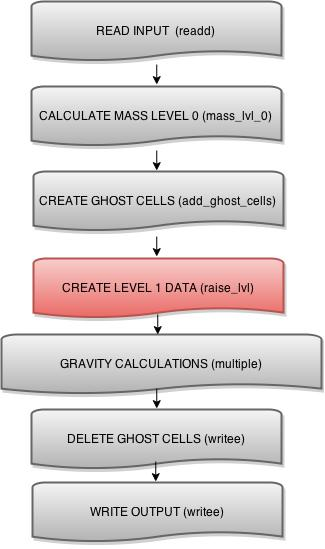
\includegraphics[width = .25\textwidth]{./Diagram4.jpg}
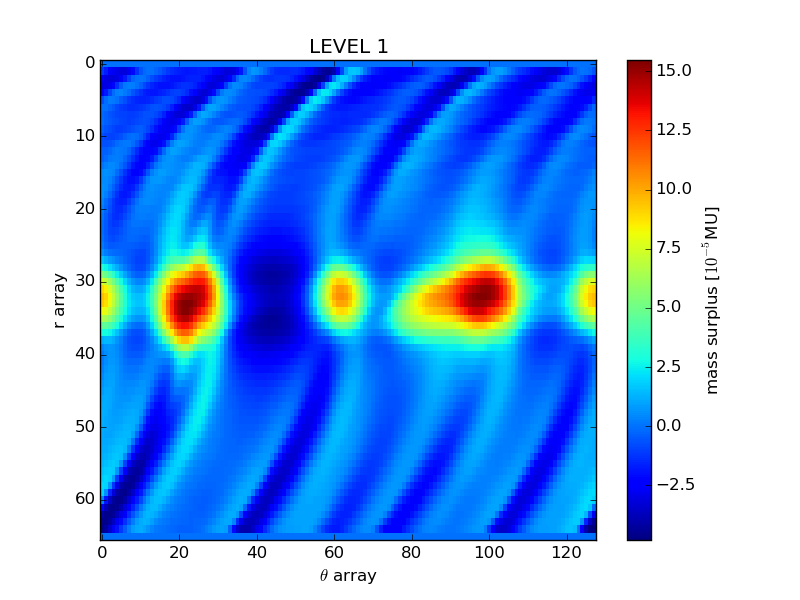
\includegraphics[width = .5\textwidth]{./mass_l1.png}
\end{figure}

\end{frame}

\begin{frame}
\frametitle{Code schema}

\begin{figure}

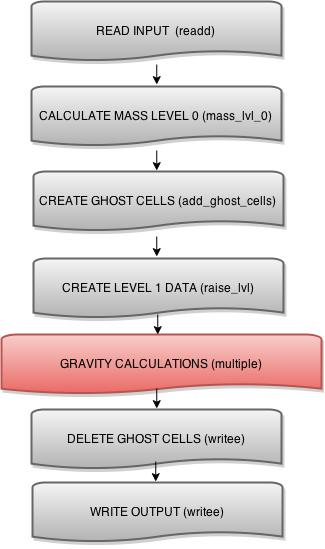
\includegraphics[width = .25\textwidth]{./Diagram5.jpg}

\end{figure}

\end{frame}

\begin{frame}
\frametitle{Code schema}

\begin{figure}


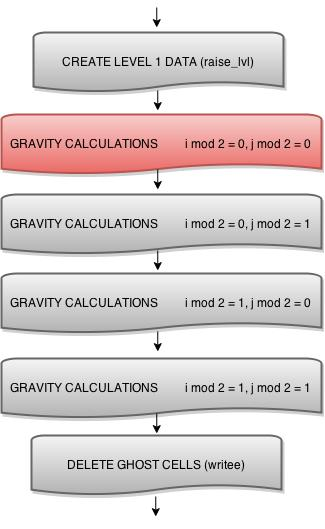
\includegraphics[width = .25\textwidth]{./Grav_Diagram1.jpg}
\end{figure}

\end{frame}




\begin{frame}
\frametitle{Code schema}

\begin{figure}

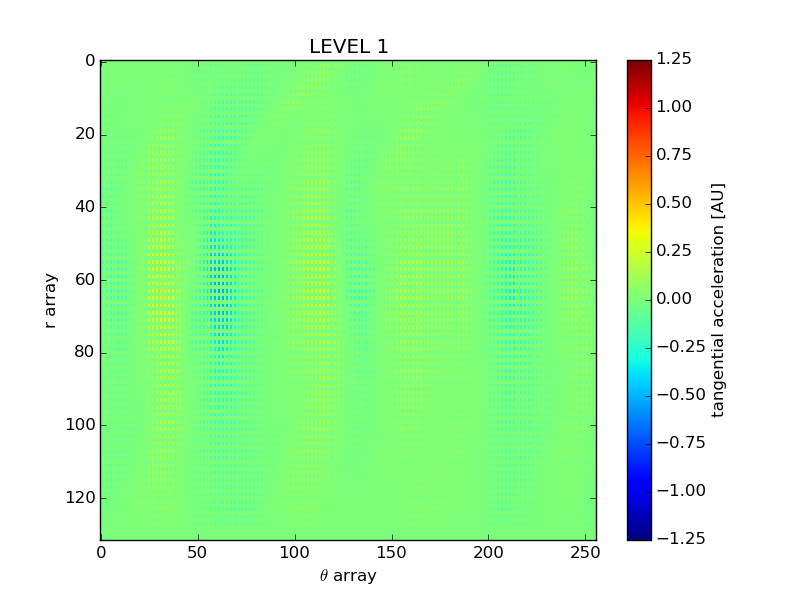
\includegraphics[width = .4\textwidth]{./level1_1_tangential.png}
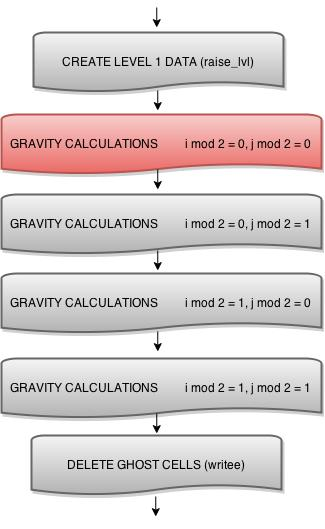
\includegraphics[width = .2\textwidth]{./Grav_Diagram1.jpg}
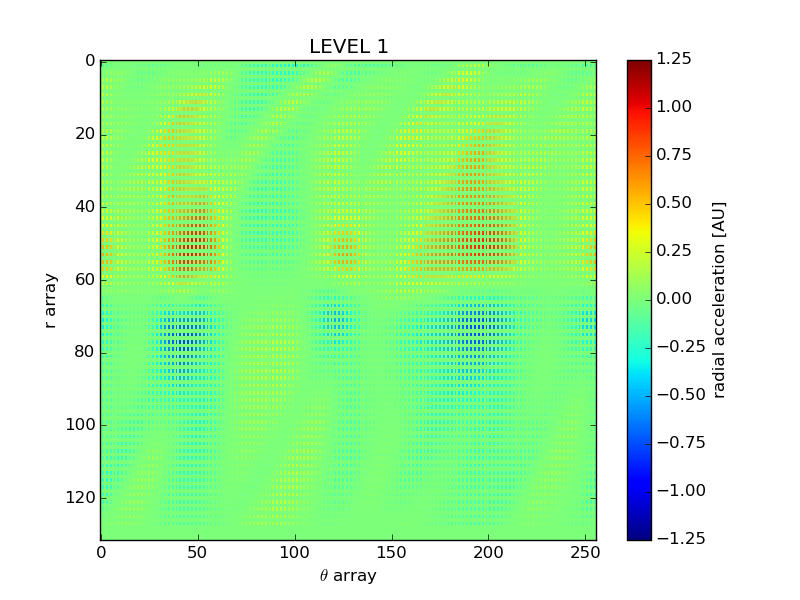
\includegraphics[width = .4\textwidth]{./level1_1_radial.png}
\end{figure}

\end{frame}

\begin{frame}
\frametitle{Code schema}

\begin{figure}

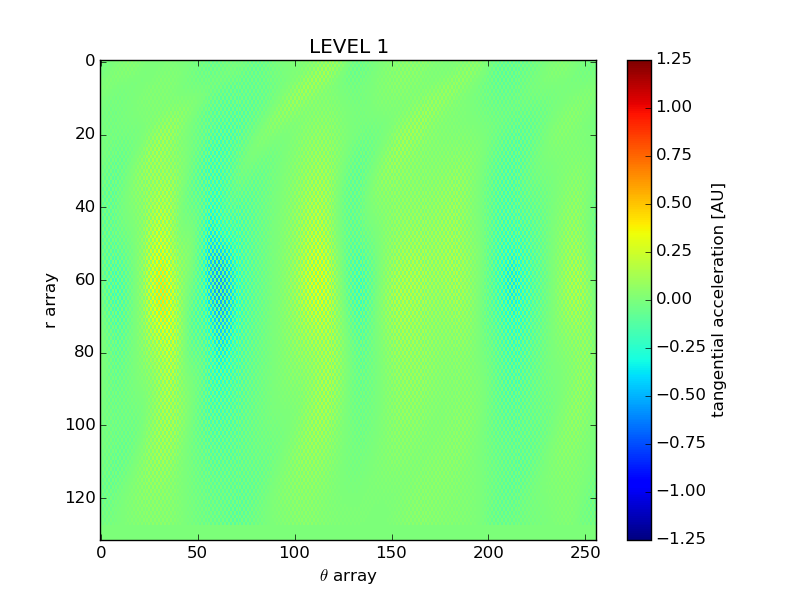
\includegraphics[width = .4\textwidth]{./level1_2_tangential.png}
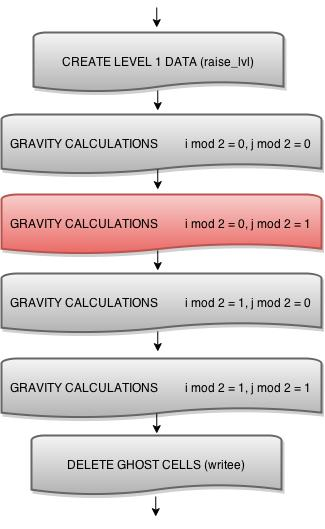
\includegraphics[width = .2\textwidth]{./Grav_Diagram2.jpg}
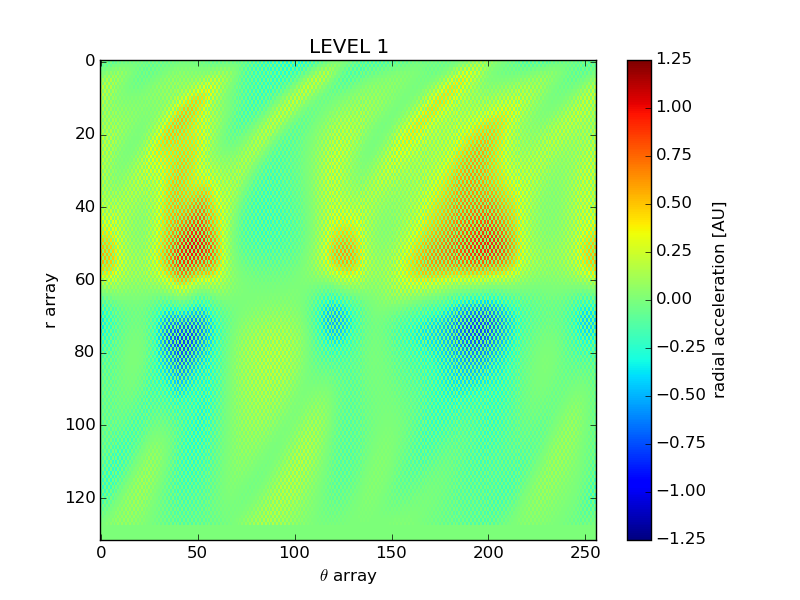
\includegraphics[width = .4\textwidth]{./level1_2_radial.png}
\end{figure}

\end{frame}

\begin{frame}
\frametitle{Code schema}

\begin{figure}

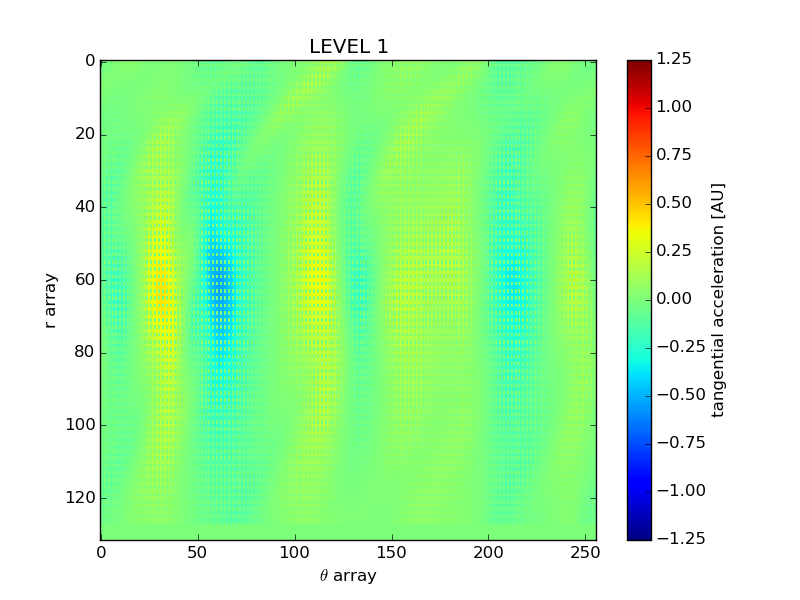
\includegraphics[width = .4\textwidth]{./level1_3_tangential.png}
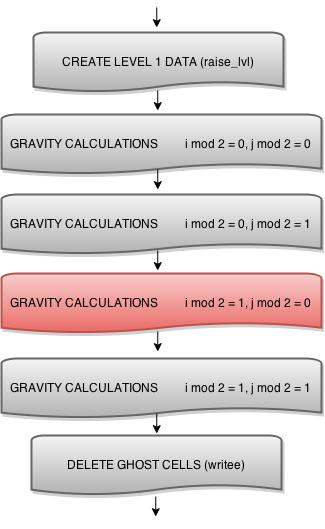
\includegraphics[width = .2\textwidth]{./Grav_Diagram3.jpg}
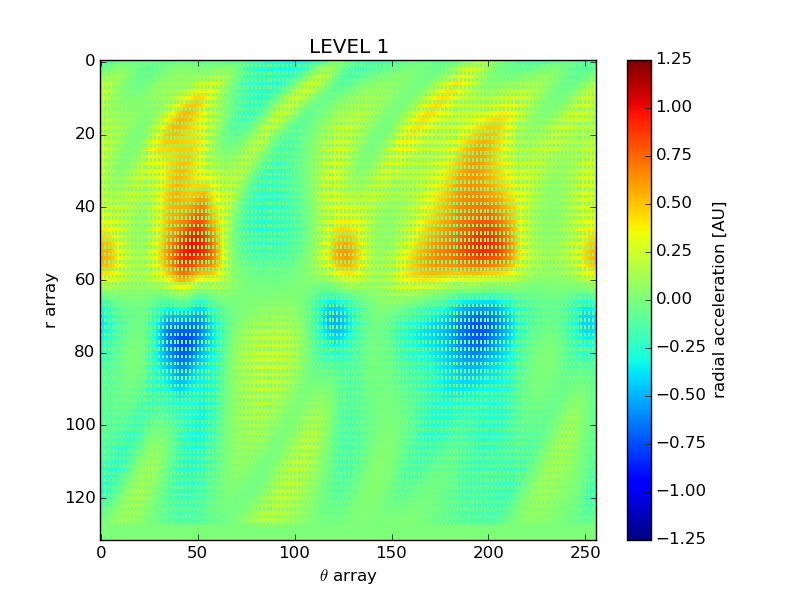
\includegraphics[width = .4\textwidth]{./level1_3_radial.png}
\end{figure}

\end{frame}

\begin{frame}
\frametitle{Code schema}

\begin{figure}

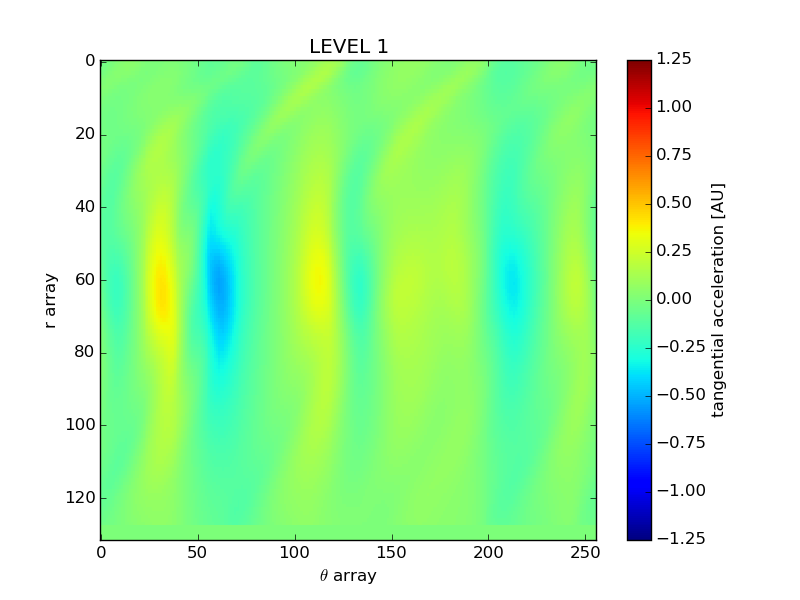
\includegraphics[width = .4\textwidth]{./level1_4_tangential.png}
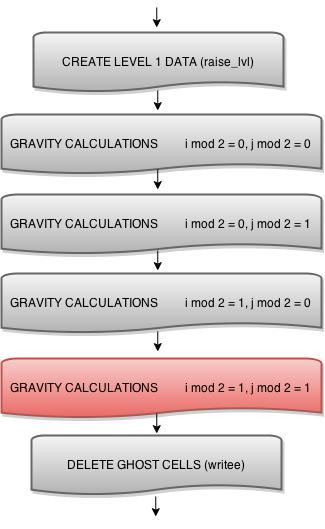
\includegraphics[width = .2\textwidth]{./Grav_Diagram4.jpg}
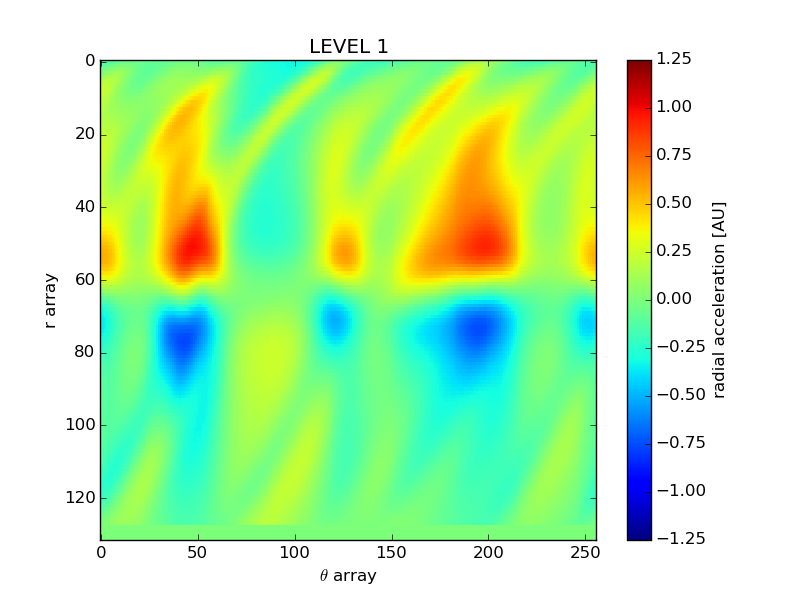
\includegraphics[width = .4\textwidth]{./level1_4_radial.png}
\end{figure}

\end{frame}

\begin{frame}
\frametitle{Code schema}
\framesubtitle{Version with refinement}

\begin{figure}

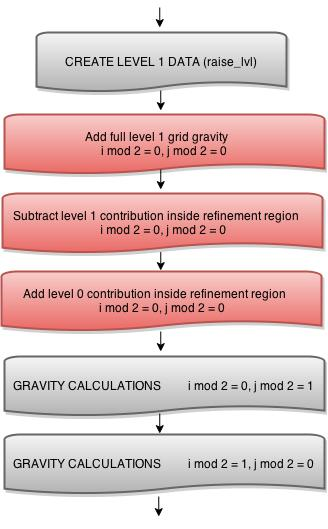
\includegraphics[width = .25\textwidth]{./3step_Diagram.jpg}
\begin{itemize}
\item avoids a series of "if" statements
\item main cpu-time usage due to the level1 full calculations
\item the larger the number of cells - the smaller the share of the other two  
\end{itemize}
\end{figure}

\end{frame}

\begin{frame}
\frametitle{Results}
\framesubtitle{LEVEL 0 vs LEVEL 1}
\begin{figure}
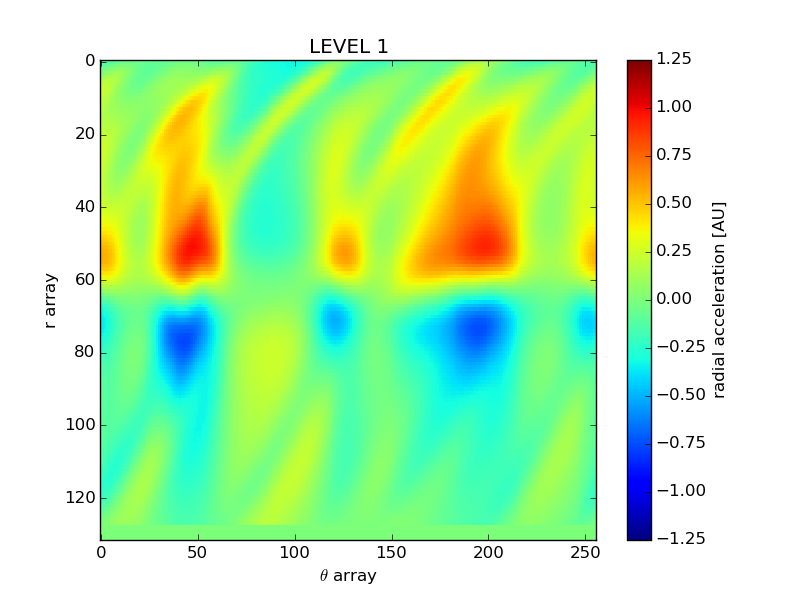
\includegraphics[width = .5\textwidth]{./level1_4_radial.png}
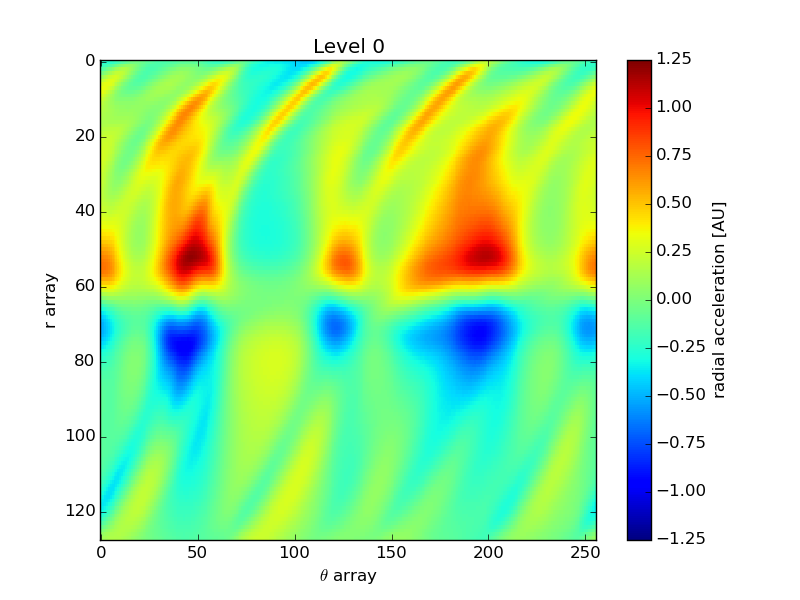
\includegraphics[width = .5\textwidth]{./level0_radial.png}
\newline
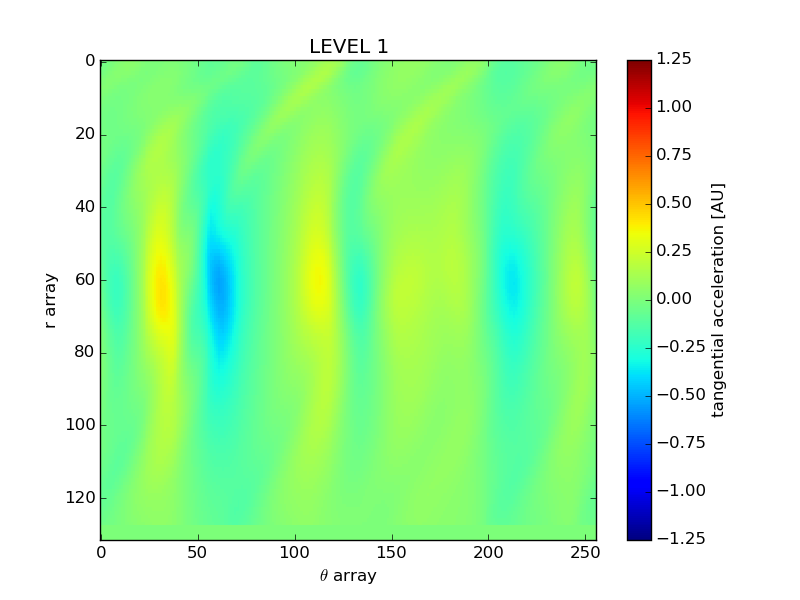
\includegraphics[width = .5\textwidth]{./level1_4_tangential.png}
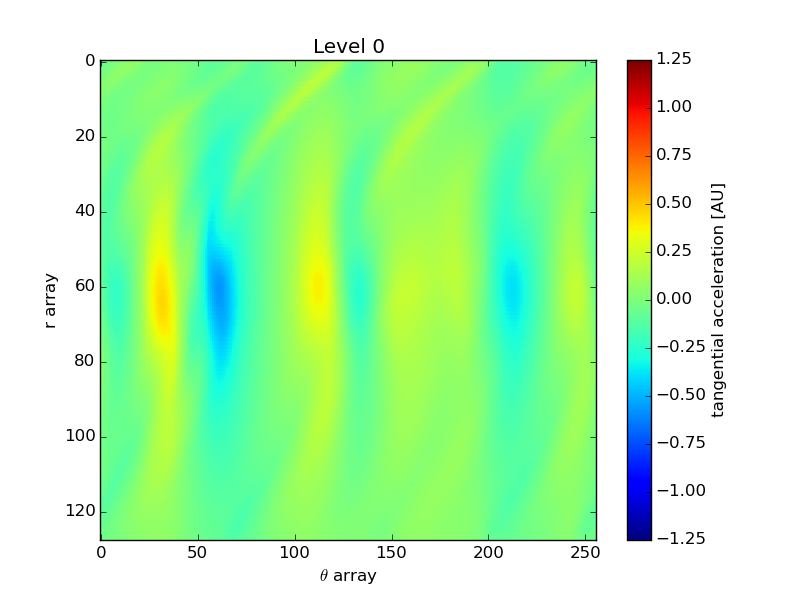
\includegraphics[width = .5\textwidth]{./level0_tangential.png}
\end{figure}

 
\end{frame}

\begin{frame}
\frametitle{Results}
\framesubtitle{LEVEL 0 vs Refined}
\begin{figure}
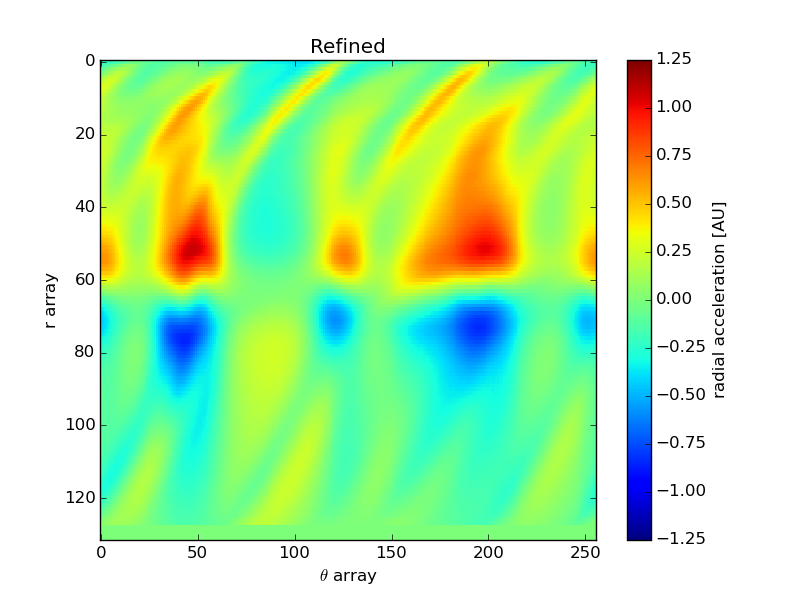
\includegraphics[width = .5\textwidth]{./ref_radial.png}
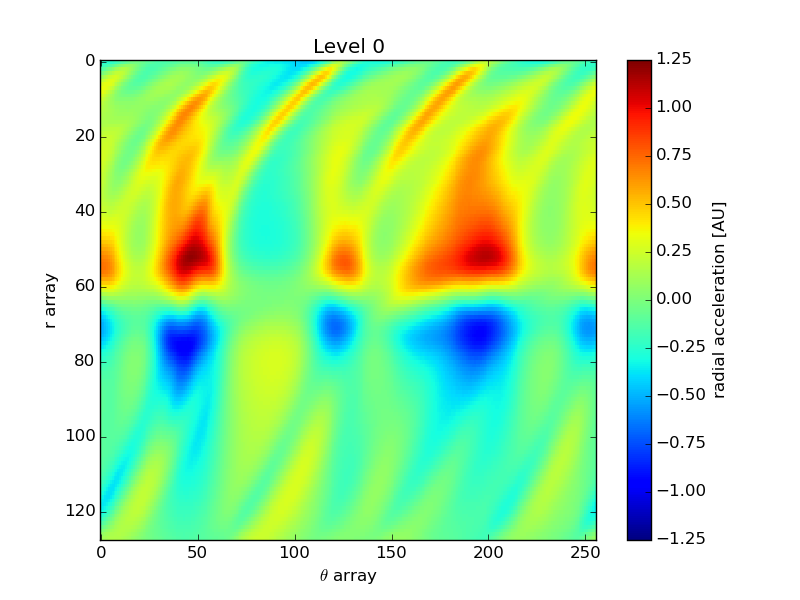
\includegraphics[width = .5\textwidth]{./level0_radial.png}
\newline
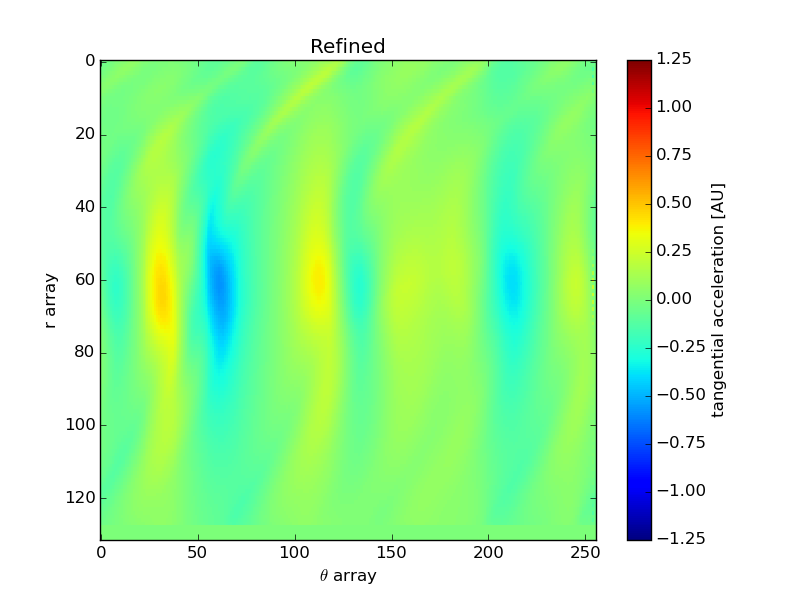
\includegraphics[width = .5\textwidth]{./ref_tangential.png}
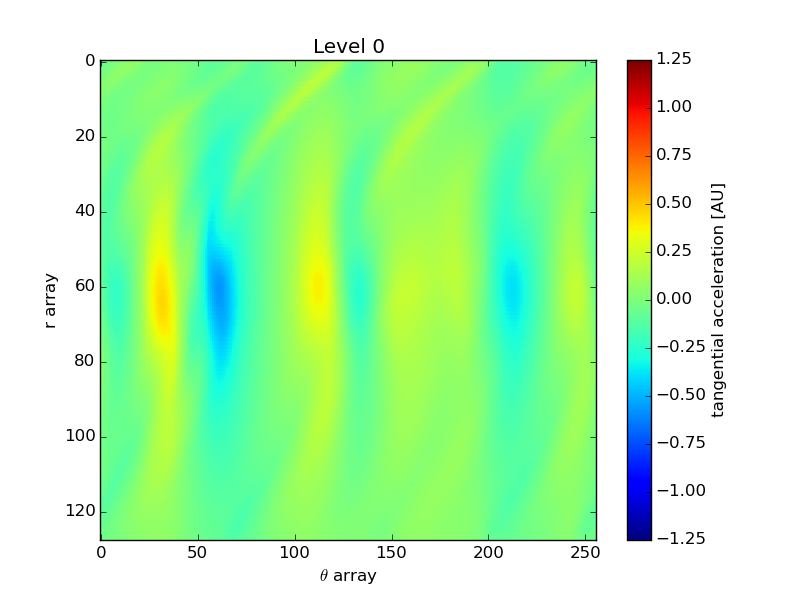
\includegraphics[width = .5\textwidth]{./level0_tangential.png}
\end{figure}

 
\end{frame}

\begin{frame}
\frametitle{Results}
\framesubtitle{LEVEL 0 vs Refined : Differences}
\begin{figure}
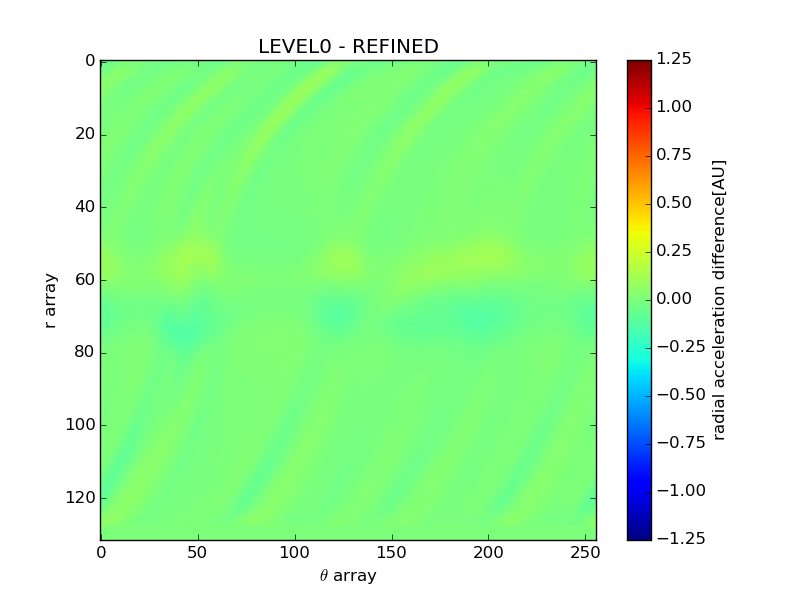
\includegraphics[width = .5\textwidth]{./diff_abs_lvl0_ref_radial.png}
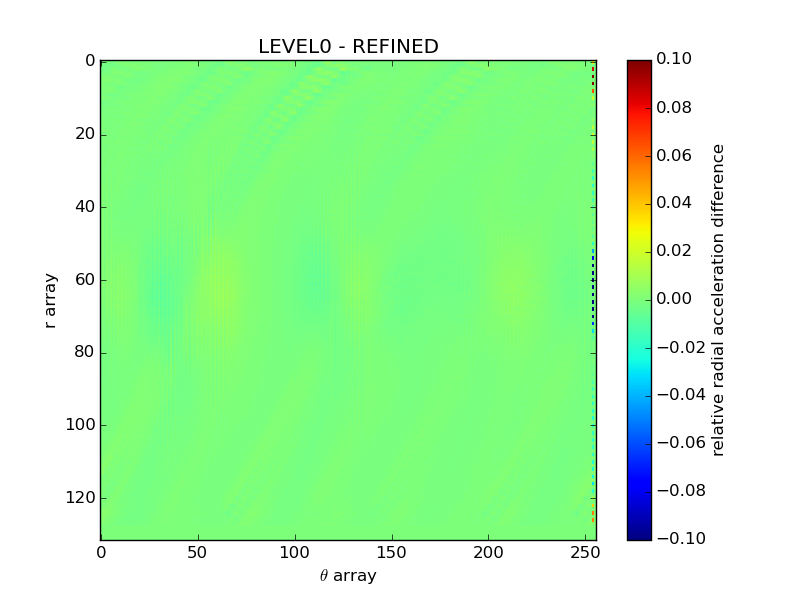
\includegraphics[width = .5\textwidth]{./diff_rel_lvl0_ref_radial.png}
\newline
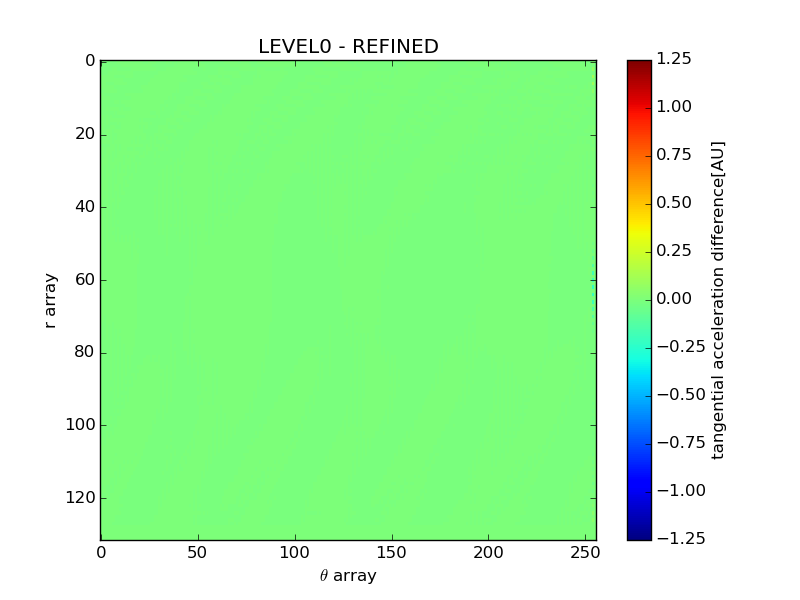
\includegraphics[width = .5\textwidth]{./diff_abs_lvl0_ref_tangential.png}
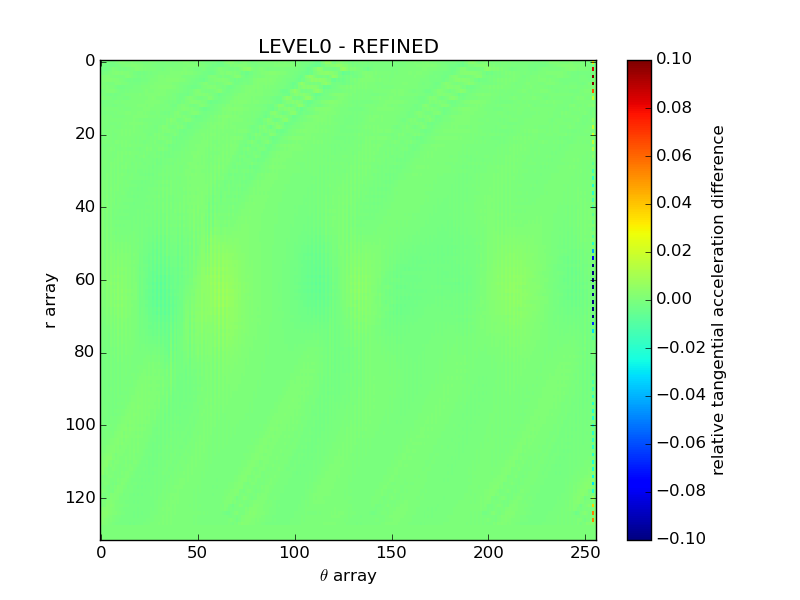
\includegraphics[width = .5\textwidth]{./diff_rel_lvl0_ref_tangential.png}
\end{figure} 
\end{frame}


\begin{frame}
\frametitle{Results}
\framesubtitle{LEVEL 0 vs Refined : Maximum differences}
\begin{figure}
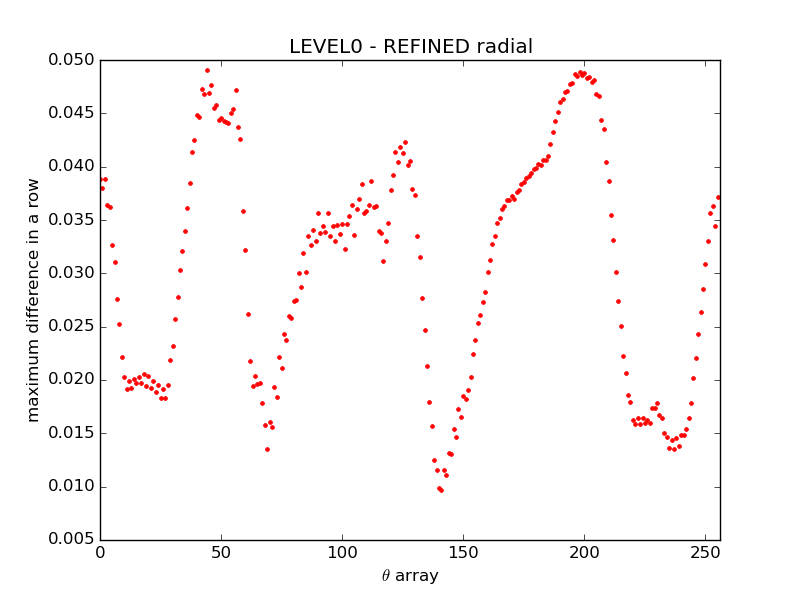
\includegraphics[width = .5\textwidth]{./1D_diff_radial.png}
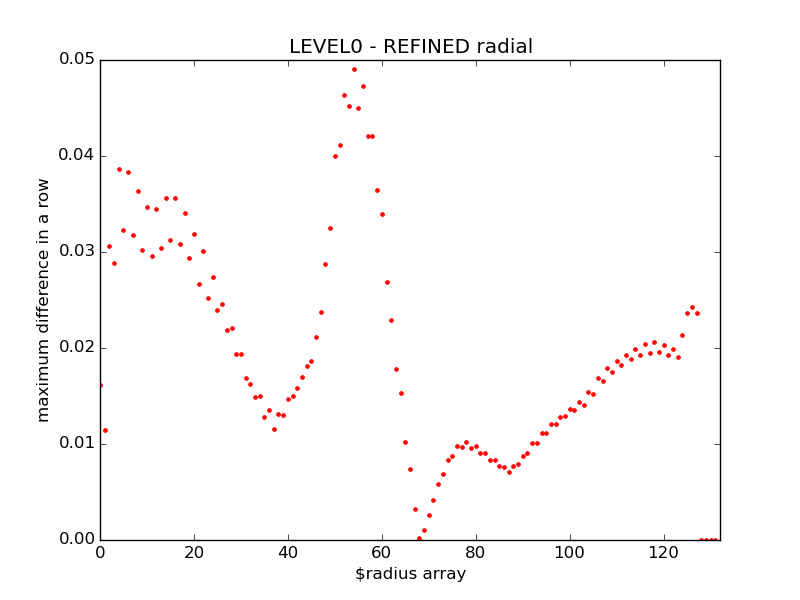
\includegraphics[width = .5\textwidth]{./1D_diff_radial_radius.png}
\newline
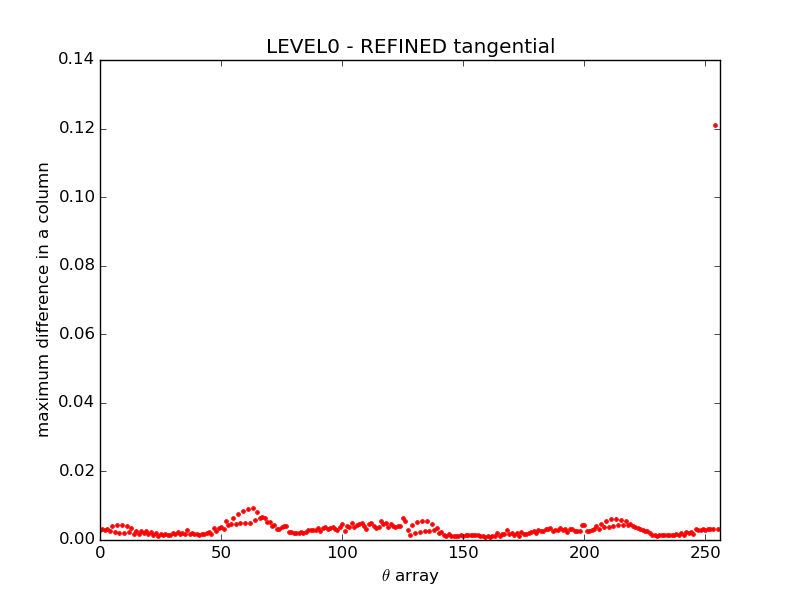
\includegraphics[width = .5\textwidth]{./1D_diff_tangential.png}
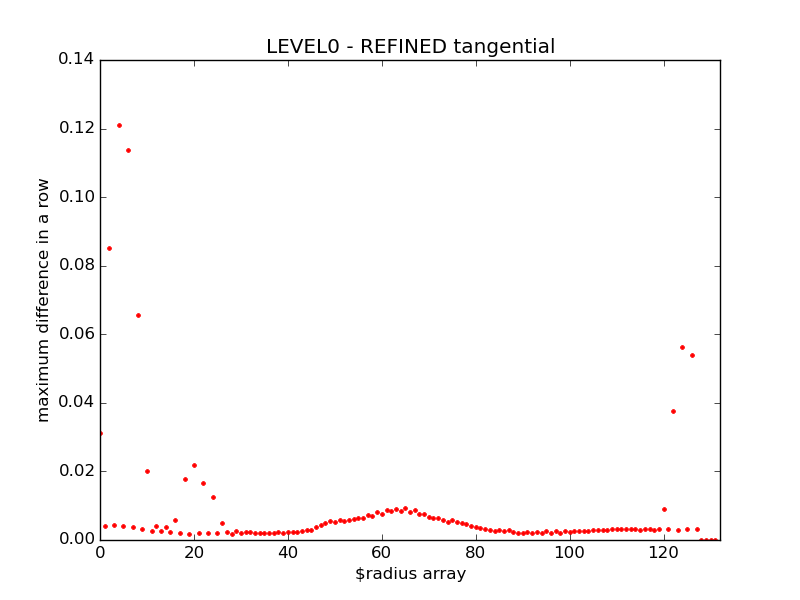
\includegraphics[width = .5\textwidth]{./1D_diff_tangential_radius.png}
\end{figure} 
\end{frame}

\begin{frame}
\frametitle{Time measurements}


\begin{itemize}
\item 16 s  level 0 optimization (March results) ;
\item 61 s  level 0 constrained for refinement method;
\item 14 s  level 1 with no refinement;
\item 15 s  level 1 with level 0 refinement;  


\end{itemize}
\end{frame}

\begin{frame}
\frametitle{Towards a faster code}
\framesubtitle{Using intra-node parallelism}

\begin{figure}

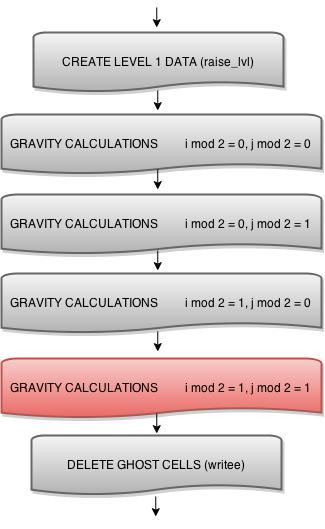
\includegraphics[width = .4\textwidth]{./Grav_Diagram4.jpg}

\end{figure}


\end{frame}

\begin{frame}
\frametitle{Towards a faster code}
\framesubtitle{Using intra-node parallelism}

\begin{figure}

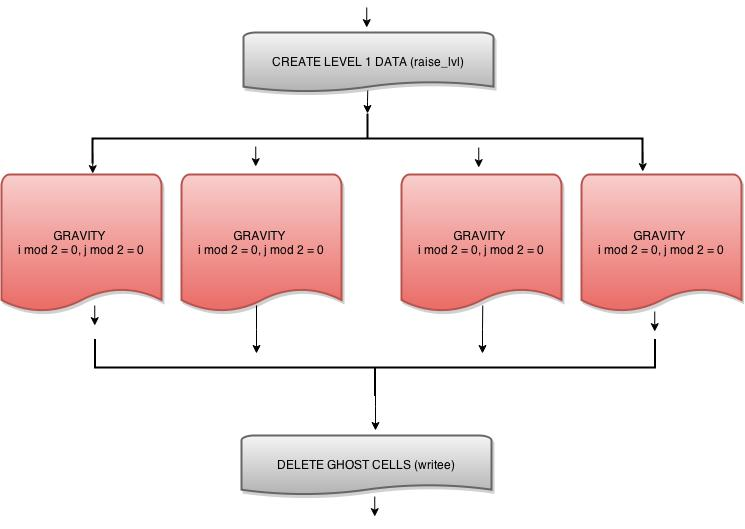
\includegraphics[width = .8\textwidth]{./Grav_Diagram_para.jpg}

\end{figure}


\end{frame}




\begin{frame}
\frametitle{Towards a faster code}
\framesubtitle{Using intra-node parallelism}

\begin{figure}

\includegraphics[width = .2\textwidth]{./Grav_Diagram_para.jpg}

\end{figure}

\begin{itemize}
\item run 4 independent tasks on shared memory ;
\item could use i.e. OpenMP;
\item simpler distribution of tasks;
\item the inter-node MPI structure would not change;  
\item no MPI communication during one step calculations.
\item reduce needed time by ~ 4 to 3-4 s


\end{itemize}


\end{frame}



\begin{frame}
\frametitle{Towards a faster code}
\framesubtitle{How about using GPUs?}

\begin{figure}
\includegraphics[width = .5\textwidth]{./cpu_gpu.png}
\caption {CPU vs GPU. (Source: NVIDIA)}
\end{figure}

\begin{itemize}
\item rewrite code in GPU languages (i.e. CUDA);
\item the gravity calculation part would stay the same;
\item the outer loops would need to be replaced to take advantage of the GPU;
\item the inter-node MPI would not change;  
\item intra-node communication problems...


\end{itemize}


\end{frame}

\begin{frame}
\frametitle{Towards a faster code;}
\framesubtitle{Movement of the industry and scientific community}

\begin{figure}
\includegraphics[width = .5\textwidth]{./unified_memory_schematic.jpg}
\caption {Future direction for hardware design. (Source: NVIDIA)}
\end{figure}

\begin{itemize}
\item avoid intra-node communication time-loss 
\item could reduce the needed time to under 1 s

\end{itemize}

\end{frame}



\begin{frame}

\frametitle{The fortran code}

\Fontvi

\lstinputlisting[basicstyle=\tiny, language = Fortran, firstline = 1, lastline = 50]{/home/ics/mihai/git/Computational_Science_II_Open/New_attempt/new.f90}



\end{frame}




\end{document}
